\newpage

\section{About Medians}
Here we explore several ways of thinking about the medians of triangles.  

\begin{prob}  
On cardstock, use a ruler to draw a medium-sized, non-right, non-isosceles triangle, and then cut it out as accurately as you can.  Draw two of the medians on the cutout triangle.  Draw the third median to make sure they are concurrent.  
\begin{enumerate}
\item Using a ruler, try balancing the triangle along each median.  (Ask a partner to hold the ruler steady.)  
\item Now try balancing the triangle along a line that is \emph{not} a median.  How does your line relate to the intersection of the medians?  Explain why this makes sense.  
\item Try balancing the triangle from a string at the intersection of the medians.  (Use the point of your compass to make a hole in the cardstock.)
\end{enumerate}

\end{prob}

\begin{prob}
Imagine stacking toothpicks in a triangle, as shown below.  

$$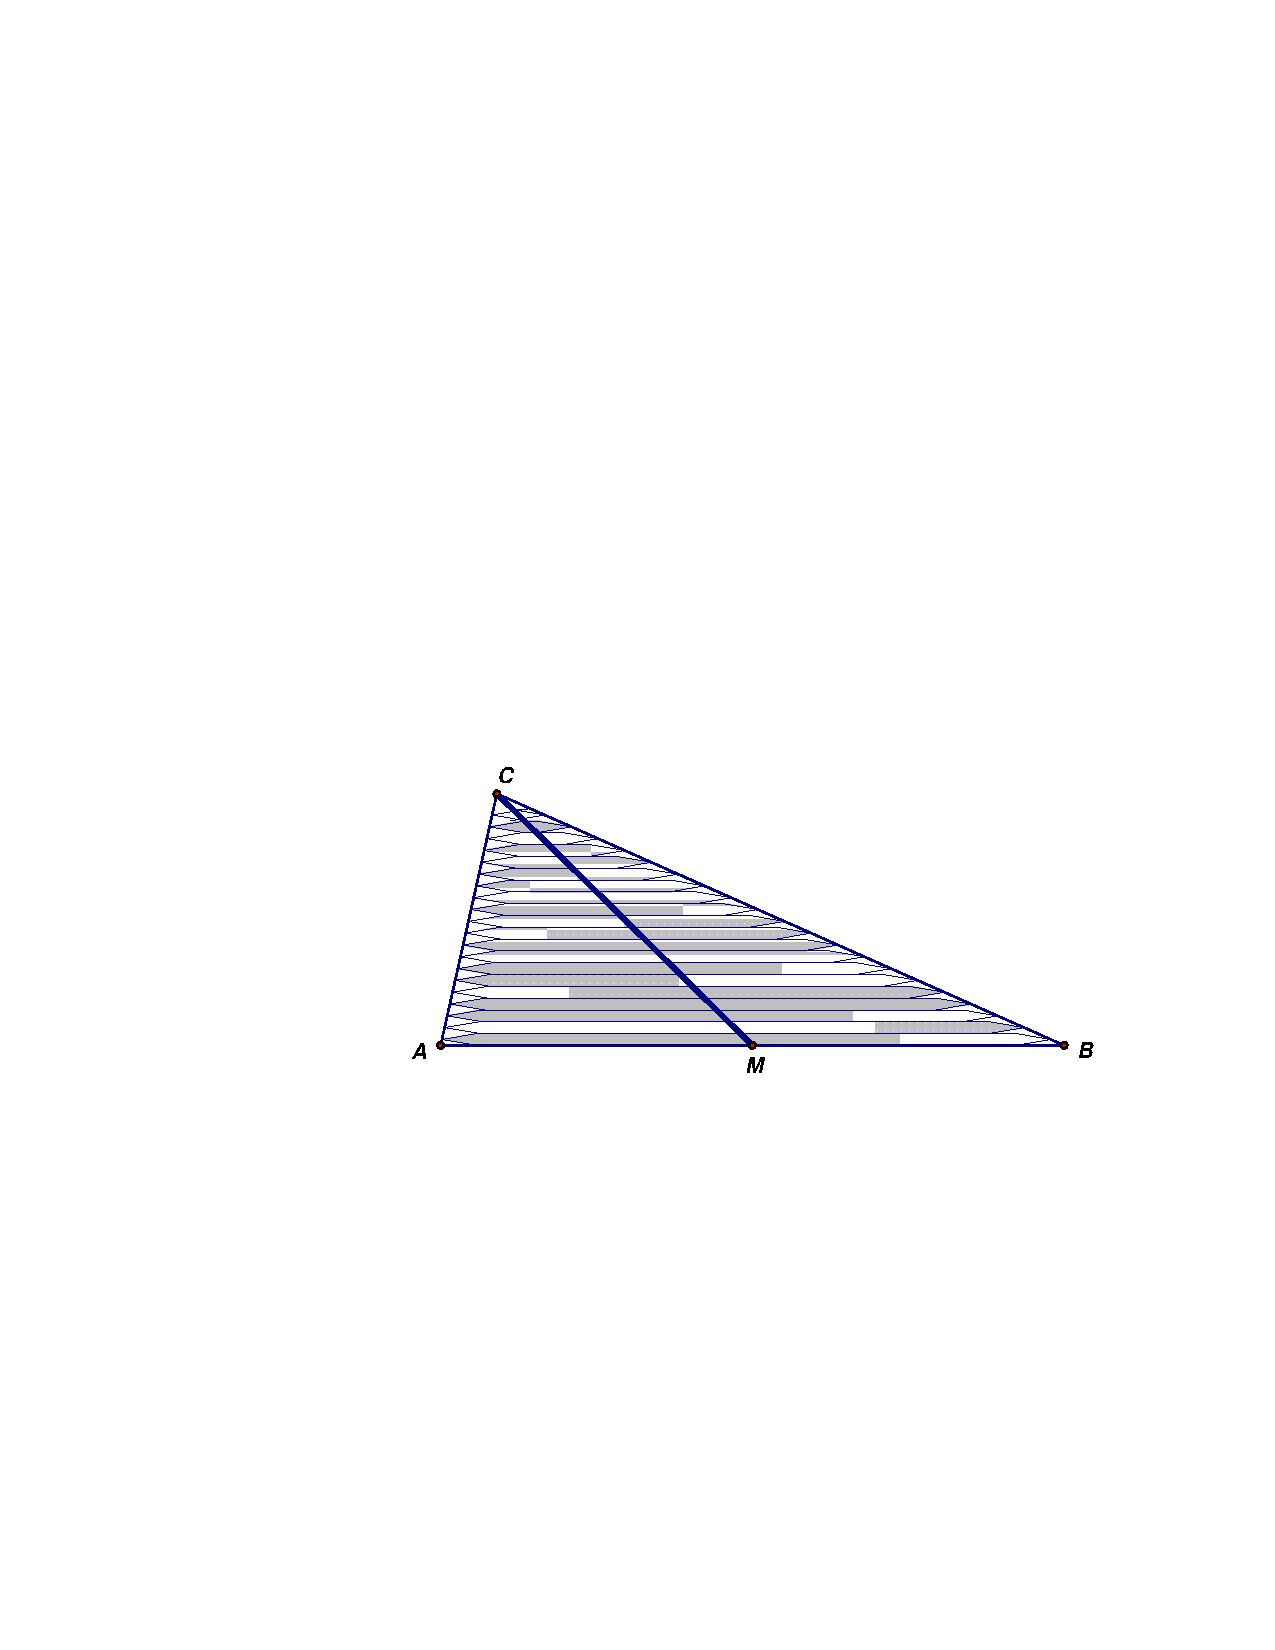
\includegraphics[width=2.5in]{Toothpicks.pdf}$$

\begin{enumerate}
\item Explain, using toothpicks, why the triangle would balance on a ruler placed along the median $\overline{CM}$.  
\item Explain, using a different collection of toothpicks, why the triangle would balance along the median to side $\overline{AC}$.  Describe how the toothpicks would need be placed, relative to side $\overline{AC}$.
\item The two medians will intersect at a point.  Explain why the triangle (without toothpicks) should balance from a string or on a pencil point at the intersection of the two medians.  
\item Use a balancing argument to explain why the third median should contain the intersection of the first two.  
\end{enumerate}
\end{prob}

\begin{prob}
Use the picture below to show that a pair of medians intersects at a point 2/3 of the way from the vertex to the opposite side.  Then use that fact to argue that the three medians must be concurrent.  
$$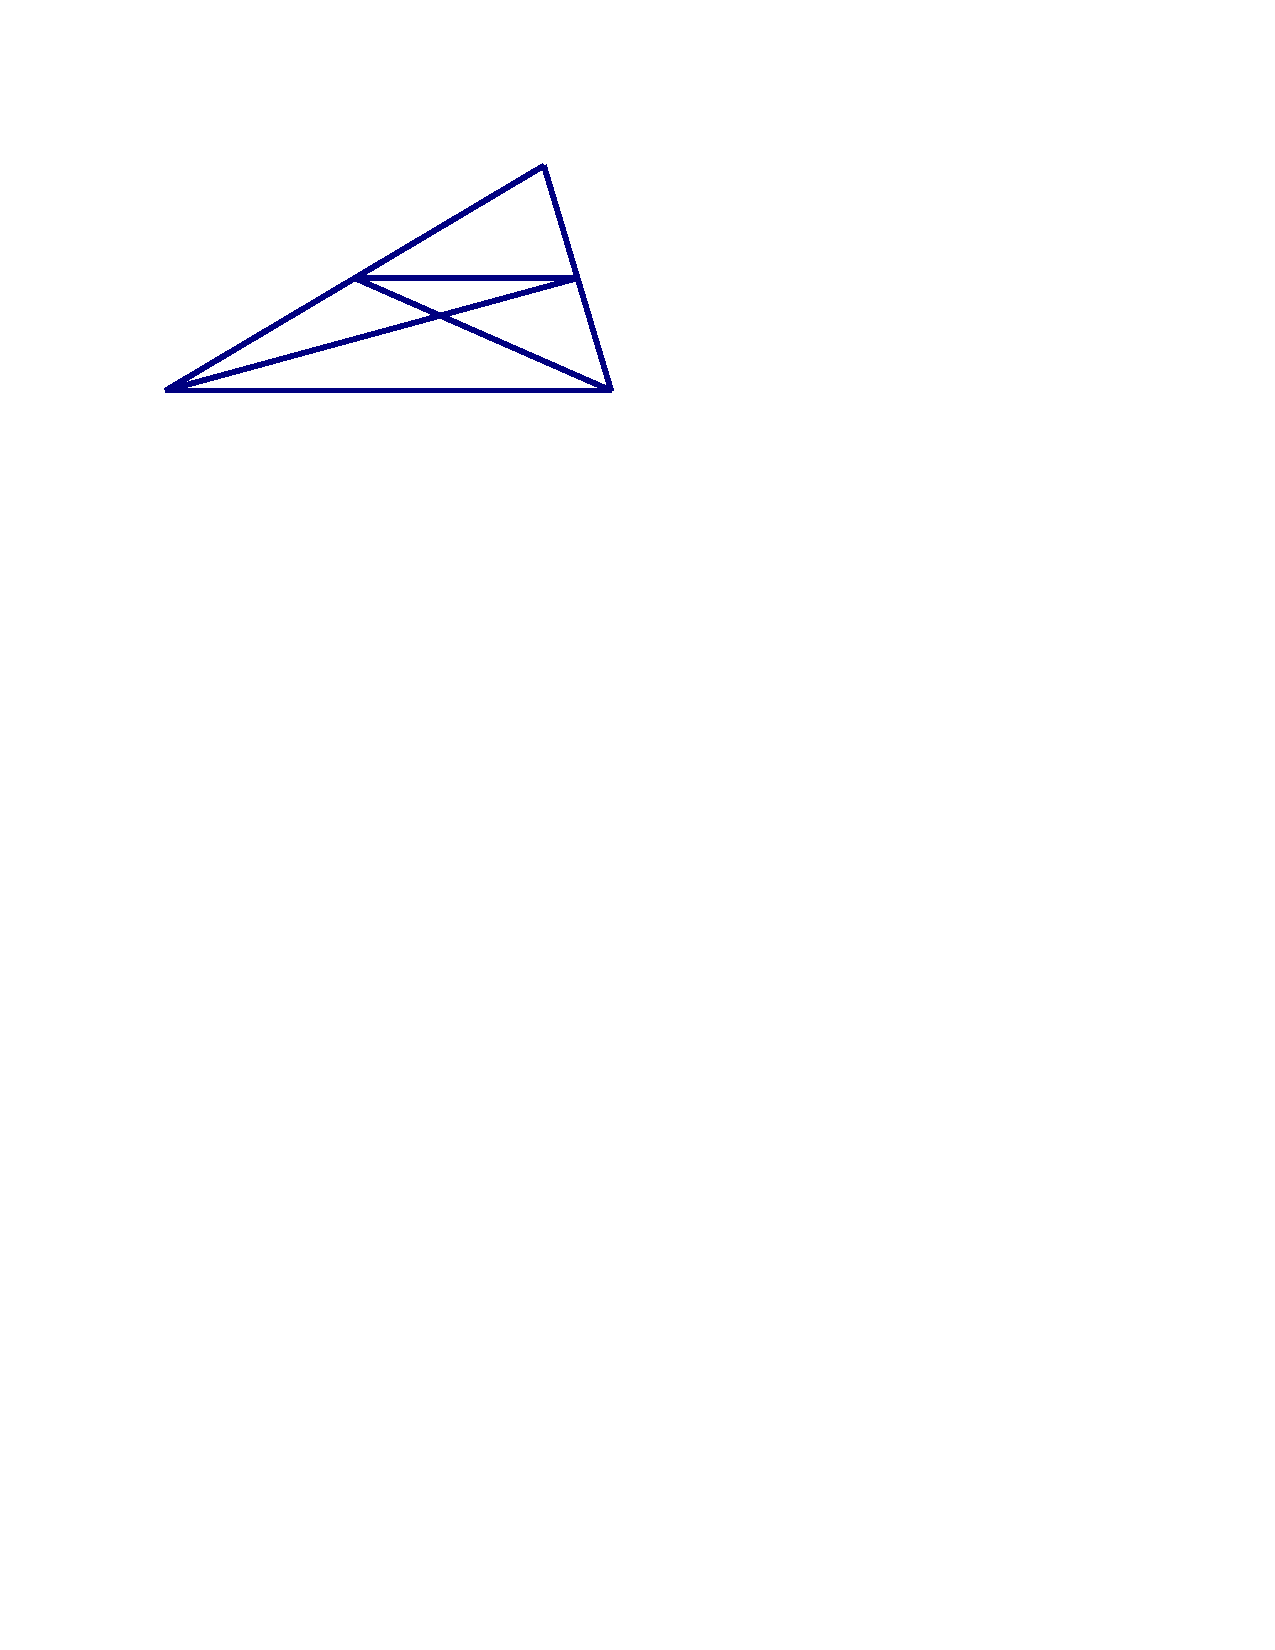
\includegraphics[width=2.5in]{median1.pdf}$$
\end{prob}

\begin{prob}
Imagine a triangle made of nearly weightless material with one-pound weights placed at each of the vertices, $A$, $B$, and $C$.  
\begin{enumerate}
\item Explain why the triangle will balance on a ruler along the median to side $\overline{AB}$.  
\item Explain why the triangle will continue to balance along the median when the masses at $A$ and $B$ are both moved to the midpoint of $\overline{AB}$.  
\item Now imagine trying to balance the triangle at a single point along the median.  Where will it balance?  Use the phrase ``weighted average'' to explain your reasoning.   
\end{enumerate}
\end{prob}

\begin{prob}
Using the picture below, explain why the medians of the large triangle are also medians of the medial triangle.  Then explain how repeating this process indefinitely proves that the medians are concurrent.
$$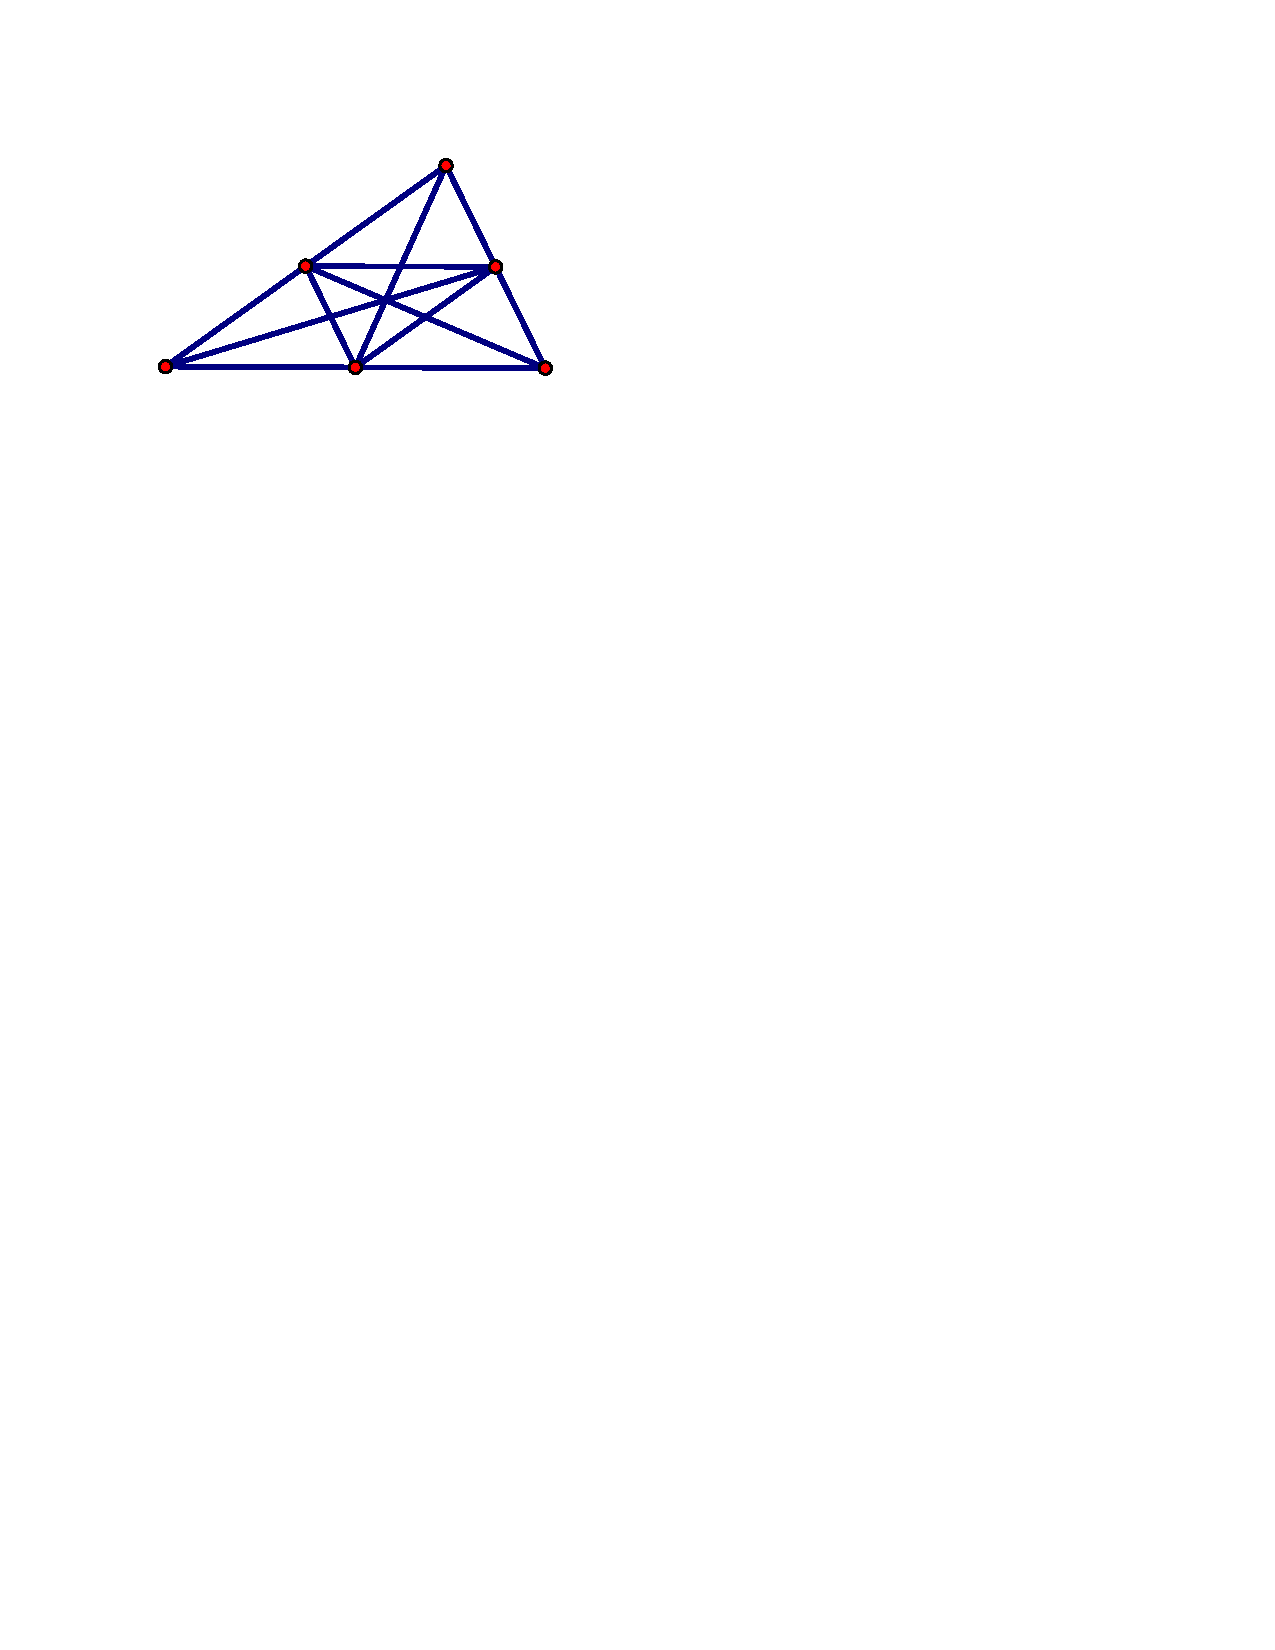
\includegraphics[width=2.5in]{median2.pdf}$$
\end{prob}
 


